% =============================================================================
%  NeuralPSI: composing a learned biometric feature extractor with fuzzy-labelled
%  private set intersection --- and measuring what the composition costs.
%
%  Build:  tectonic -X compile paper.tex
%  The long exploratory draft this replaces is kept at draft-long.tex as source
%  material; it is not part of the submission.
% =============================================================================
\documentclass[runningheads]{llncs}

\usepackage[T1]{fontenc}
\usepackage{amsmath,amssymb}
\usepackage{booktabs}
\usepackage{graphicx}
\usepackage{xcolor}
\usepackage[hidelinks]{hyperref}

\graphicspath{{figures/}}

% allow denser pages: default LaTeX bails to a float page early
\renewcommand{\topfraction}{0.9}
\renewcommand{\bottomfraction}{0.8}
\renewcommand{\textfraction}{0.07}
\renewcommand{\floatpagefraction}{0.8}

\newcommand{\xt}{\tilde{\mathbf{x}}}
\newcommand{\yt}{\tilde{\mathbf{y}}}
\newcommand{\Fnpsi}{\mathcal{F}_{\mathsf{NeuralPSI}}}

\begin{document}

\title{Fuzzy-Labelled PSI for Biometric Authentication:\\
       A Composition and Its Costs}

\author{Anonymous Author}
\authorrunning{Anonymous}
\institute{Anonymous Institution}

\maketitle

\begin{abstract}
Privacy-preserving biometric authentication at scale is usually built on homomorphic
encryption, which keeps templates encrypted but pays large key material and a structural
packing ceiling. Fuzzy-labelled private set intersection (FLPSI) avoids both, but matches
only binary strings under Hamming distance. We study what happens when the two halves are
joined: a Siamese CNN feature extractor run locally in plaintext, a fixed public Super-Bit
projection binarising its 16-dimensional embedding into a 128-bit code, and FLPSI as the
matcher. We implement the composition and measure it on SOCOFing, where it reaches
1.89\% equal-error rate (95\% CI [1.56, 2.20]) against a 0.33\% floating-point ceiling
with 16-byte server-side
templates and no 117\,MB rotation key. We then report what the composition costs. The
central finding is a measurement: the FLPSI error analysis assumes impostor codes are
uniform, but codes derived from a 16-dimensional embedding carry roughly 16 degrees of
freedom, and their Hamming distribution has $3.6\times$ the assumed standard deviation
while having \emph{exactly} the assumed mean --- so the discrepancy is invisible to any
first-moment check. At the published parameters this makes the per-record false-accept
rate $1{,}550\times$ larger than predicted, and no setting of the sub-sampling parameters
repairs it, because distinct fingers collide on identical codes at a rate of
$2.8\times10^{-6}$ that lower-bounds every parameterisation. We give the measured
frontier, show multi-finger fusion is the only effective remedy, formalise the leakage
with simulators for both corruptions, and show the stored code is a bearer credential
failing all three ISO/IEC 24745 template-protection requirements.

\keywords{Private set intersection \and Biometric template protection \and
Locality-sensitive hashing \and Secure computation \and ISO/IEC 24745.}
\end{abstract}

\section{Introduction}
\label{sec:intro}

In 2015 the United States Office of Personnel Management disclosed that attackers had
exfiltrated the records of 21.5 million people, including 5.6 million
fingerprints~\cite{Gootman16}. The passwords in that breach were reset within days. The
fingerprints could not be: a compromised biometric is compromised permanently. This
asymmetry is why ISO/IEC 24745~\cite{ISO24745} requires three properties of any stored
biometric reference --- \emph{irreversibility}, so the reference cannot be inverted to the
biometric; \emph{unlinkability}, so references for the same subject in different databases
cannot be correlated; and \emph{renewability}, so a compromised reference can be replaced
by a fresh one derived from the same trait.

Systems that keep templates encrypted end-to-end address the first requirement directly.
Blind-Touch~\cite{ChoiWooKim24} is the current reference point: it evaluates the matching
step under CKKS~\cite{CKKS17} so that the server never sees a plaintext template. The
guarantee is strong, and the costs are structural rather than incidental. A 117\,MB Galois
rotation key must be distributed to every client; each query ciphertext is 856\,KB; and
because the scheme packs 512 users into one ciphertext, the database is organised around a
slot-packing ceiling rather than around the workload.

Fuzzy private set intersection offers a different trade. Fuzzy-labelled PSI
(FLPSI)~\cite{BuiCong25} lets a client learn the label attached to any server record
within Hamming distance $\tau$ of its query, at communication linear in the database and
with no key material of consequence. But FLPSI matches \emph{bit-strings}, and a
fingerprint is not a bit-string. Bridging that gap --- turning a noisy image into a short
binary code whose Hamming distance tracks biometric similarity --- is the missing piece.

\paragraph{This paper.} We build the bridge and measure what it costs. A Siamese CNN runs
\emph{on the client, in plaintext}, producing a 16-dimensional embedding; a fixed, public,
training-free Super-Bit projection~\cite{JiEtAl12} binarises it to a 128-bit code; FLPSI
matches the code and returns a label. The design removes the homomorphic layer entirely:
server-side templates are 16 bytes, there is no rotation key, and there is no packing
ceiling.

That is the easy half, and on its own it would be an engineering note. The substance of this
paper is what we found on measuring the composition against the error model its cryptographic
half assumes.

FLPSI's parameters are chosen from a model in which impostor codes are uniform, so the Hamming
distance between unrelated records is $\mathrm{Binomial}(128,\tfrac12)$ with standard deviation
$5.66$. Codes from our bridge --- and, we argue, from any LSH bridge over a learned embedding ---
are not uniform: they are 128 projections of a 16-dimensional vector, so they carry roughly 16
degrees of freedom and inherit the embedding's angular distribution, including the fact that some
fingers genuinely look alike. Over $2.88\times10^{6}$ held-out impostor pairs, the mean impostor distance is $64.0$ --- \emph{exactly} what the model
predicts, because the quantiser balances each bit. The standard deviation is $20.22$,
$3.6\times$ the assumed value. A first-moment sanity check on the codes passes cleanly
while the analysis underlying the parameter choice is wrong by three orders of magnitude:
at the published operating point the per-record false-accept rate is
$4.58\times10^{-2}$ rather than the predicted $2.95\times10^{-5}$.

Nor is this a tuning problem. We sweep 6{,}848 parameter combinations and find none that
reaches even a $10^{-2}$ query-level false-accept rate at $N = 5{,}000$ without rejecting
most legitimate users. The reason is a floor: 8 of our $2.88\times10^{6}$ impostor pairs
produce \emph{identical} 128-bit codes, a rate of $2.8\times10^{-6}$ that no choice of
sub-sampling parameters can go below, since a zero-distance pair is accepted by every
parameterisation. This bound is a property of the code, not of the protocol.

\paragraph{Contributions.}
\begin{description}\itemsep2pt
\item[C1.] A design that decouples perceptual feature extraction (client-side, plaintext)
from private matching (FLPSI), removing the homomorphic-encryption layer, its 117\,MB
rotation key and its slot-packing ceiling, and returning the matched identity rather than
a similarity score (\S\ref{sec:design}).

\item[C2.] A public, training-free quantisation bridge whose interface contract with a
fuzzy-PSI matcher is stated \emph{and measured}: bit balance, inter-bit dependence, and
the empirical sub-sample collision probability against its hypergeometric prediction. We
show the bridge costs $+1.55$ percentage points of EER and that the 16-dimensional
embedding, not the code length, is the accuracy ceiling (\S\ref{sec:design},
\S\ref{sec:eval}).

\item[C3.] A parameter-selection analysis for threshold-PSI biometric matching computed
from the \emph{measured} code distribution rather than a uniform idealisation: the
$1{,}550\times$ false-accept gap, the irreducible collision floor, the measured
$(w,\theta,N)$ frontier, and multi-finger fusion as the only mechanism that crosses the
floor (\S\ref{sec:params}).

\item[C4.] A semi-honest security analysis with an explicit ideal functionality, a formal
leakage function, simulators for both corruptions and a hybrid sequence, together with an
assessment of the stored template against ISO/IEC 24745 --- including two attacks we do
not mitigate and the cost of the mitigations we propose (\S\ref{sec:security}).

\item[C5.] A prototype and its measurements: accuracy with identity-level bootstrap
confidence intervals and DET curves across three degradation levels, a bit-budget-matched
comparison against ITQ, communication and latency at the corrected operating point, and a
two-shard scaling experiment (\S\ref{sec:eval}).
\end{description}

\paragraph{What we do not claim.} We do not claim the measured error rates are acceptable
for $1{:}N$ identification at the database sizes we tested; \S\ref{sec:params} shows they
are not. We do not claim at-rest confidentiality against a compromised server. We do not
claim security against malicious adversaries. We report a composition that is attractive
on storage, key material and scaling structure, and that fails on error rates and template
protection, and we quantify both halves.

\section{Preliminaries}
\label{sec:prelim}

\subsection{Notation}

\begin{table}[h]
\centering
\caption{Notation. Symbols are used consistently throughout; in particular $d$ always denotes
the code length and never a distance bound.}
\label{tab:notation}
\small
\begin{tabular}{@{}llll@{}}
\toprule
$d$ & code length, $=128$ & $N$ & database size (records) \\
$T$ & sub-samples per query, $=64$ & $w$ & positions per sub-sample mask \\
$\theta$ & sub-sample collisions to accept & $t$ & mismatches tolerated per sub-sample \\
$H$ & Hamming distance between codes & $q(H)$ & per-sub-sample collision probability \\
$\mathbf{e}\in\mathbb{R}^{16}$ & CNN embedding & $\xt,\yt\in\{0,1\}^{d}$ & client, server codes \\
$\mathbf{P},\boldsymbol{\mu},\boldsymbol{\tau}$ & public quantiser constants &
  $m_j$ & the $j$-th sub-sampling mask \\
$\ell_i$ & label of record $i$ & $\mathbb{F}$ & field for secret sharing \\
$\lambda,\kappa$ & computational, statistical security & $S_i$ & colliding mask set for record $i$ \\
\bottomrule
\end{tabular}
\end{table}

\subsection{Homomorphic encryption, and why we leave it}

CKKS~\cite{CKKS17} supports approximate arithmetic on encrypted vectors of reals, packing many
slots into one ciphertext; rotating between slots, which any inner product needs, requires Galois
keys that dominate key material. Blind-Touch~\cite{ChoiWooKim24} applies this to fingerprint
matching, giving strong confidentiality at the cost of a 117\,MB Galois key per client, 856\,KB
per query ciphertext, and a database organised around a 512-users-per-ciphertext packing limit.

\subsection{Siamese feature extraction}

A Siamese network~\cite{ChoiWooKim24,KimOhKim20,YangEtAl20} maps two images through a shared
convolutional trunk trained so that same-identity pairs land close. We reuse this unchanged: the
trunk produces $\mathbf{e} \in \mathbb{R}^{16}$, trained with pairwise binary cross-entropy on
identity-disjoint splits. The architecture is not a contribution here; what matters is only that
the output is a low-dimensional real vector whose cosine similarity tracks identity.

\subsection{Fuzzy-labelled PSI}
\label{sec:flpsi-prelim}

Fuzzy-labelled PSI~\cite{BuiCong25} lets a client holding $\xt \in \{0,1\}^{d}$ learn the label
$\ell_i$ of any server record $\yt_i$ within a Hamming ball of the query, while the server learns
nothing. \emph{The construction is due to Bui and Cong; we use it as a black box and restate only
what our parameter analysis in \S\ref{sec:params} depends on.} It composes two primitives.

A \textbf{masked OPRF} lets the two parties evaluate a keyed PRF on sub-sampled positions of
their inputs, so that equality of the PRF images certifies equality on those positions without
revealing the underlying bits. The parties agree on $T$ public masks $m_j \in \{0,1\}^{d}$ of
weight $w$; sub-sample $j$ of a code is its restriction to the positions selected by $m_j$.

A \textbf{threshold labelled PSI} then converts collisions into a label. The server splits each
$\ell_i$ into Shamir shares~\cite{Shamir79} with reconstruction threshold $\theta$, attaches one
share per mask, and delivers them through a polynomial encoding evaluated obliviously via vector
ring-OLE, itself built from silent VOLE~\cite{BoyleEtAl19,RindalSchoppmann21} under LPN. A client
whose code collides on at least $\theta$ masks recovers $\theta$ shares and reconstructs
$\ell_i$; a client with fewer collisions learns nothing about it. Two codes at Hamming distance
$H$ therefore collide on a given mask with probability $q(H) = \binom{d-H}{w}/\binom{d}{w}$, and
acceptance follows a binomial tail --- the model we develop and test in \S\ref{sec:params}.

Communication is linear in $N$ with no packing ceiling, and the only key material is a PRF key
held by the server.

\subsection{Binary codes from real vectors}

SimHash~\cite{Charikar02} maps a vector to the signs of random hyperplane projections; for unit
vectors at angle $\vartheta$ a random hyperplane separates them with probability $\vartheta/\pi$,
so normalised Hamming distance estimates $\vartheta/\pi$ without bias. \textbf{Super-Bit
LSH}~\cite{JiEtAl12} orthonormalises the projections in blocks equal to the input dimension,
which leaves the estimator unbiased while strictly reducing its variance at the acute angles that
separate genuine from impostor pairs; at block size one it degenerates to SimHash.
\textbf{ITQ}~\cite{GongLazebnik11} instead learns a rotation minimising quantisation loss, and is
data-dependent. We use Super-Bit and compare against ITQ at a matched bit budget in
\S\ref{sec:eval}.

\section{Threat Model and Goals}
\label{sec:threat}

\paragraph{Parties and inputs.} A \emph{client} device holds a freshly captured fingerprint and
runs the feature extractor and quantiser locally, producing $\xt \in \{0,1\}^{d}$. A
\emph{server} holds a database $D = \{(\yt_i, \ell_i)\}_{i \in [N]}$ of enrolled codes and their
labels, plus a PRF key $k$. The client learns the labels of matching records; the server learns
nothing. The ideal functionality realising this is stated as
$\Fnpsi$ in \S\ref{sec:functionality}, and what the protocol leaks beyond it is stated as
$\mathcal{L}$ in \S\ref{sec:leakage} --- we defer both to the security section so they can be
read next to the proof.

\paragraph{Adversary.} We assume a \emph{semi-honest} adversary with static corruption of one
party: it follows the protocol but tries to infer more than its output. Malicious security is out
of scope (\S\ref{sec:security}). We assume the standard LPN and PRF assumptions underlying the
sub-protocols.

\paragraph{Goals.}
\begin{description}\itemsep2pt
\item[G1. Query confidentiality.] The server does not learn $\xt$, nor the biometric behind it.
\item[G2. Database confidentiality.] The client learns no more than $\mathcal{L}_{\mathsf{C}}$ of
      \eqref{eq:leakC} --- which is \emph{more} than ``the matched label'', and we say so rather
      than claiming otherwise.
\item[G3. Scale.] Cost linear in $N$, with no per-client key material of consequence and no
      structural packing ceiling.
\end{description}

\paragraph{Deployment assumptions, stated explicitly.} Three assumptions do real work and are
easy to leave implicit.

\emph{Sensor attestation.} The extractor and quantiser run on the client in plaintext by design.
From the server's perspective $\xt$ is therefore a $d$-bit string the client chose, and nothing
in the protocol binds it to a live finger. Deployments must attest the sensor; without that, the
system's security is bounded by the code-guessing analysis of \S\ref{sec:attacks} rather than by
biometric entropy.

\emph{Rate limiting.} Per-account \emph{and} per-relying-party limits are required. We show in
\S\ref{sec:attacks} that they do not mitigate the strongest attack at large $N$, which succeeds
on the first attempt; they are necessary, not sufficient.

\emph{Templates at rest.} The protocol protects data in transit. The stored code is a separate
question with a worse answer, analysed against ISO/IEC 24745 in \S\ref{sec:atrest}. We treat full
at-rest confidentiality against a compromised server as out of scope and state the resulting
limitation plainly rather than resolving it.

\paragraph{Out of scope.} Liveness detection and presentation-attack detection; malicious-model
security; side channels on the client device; and availability.

\section{System Design}
\label{sec:design}

\subsection{Architecture}

\begin{figure}[htbp]
\centering
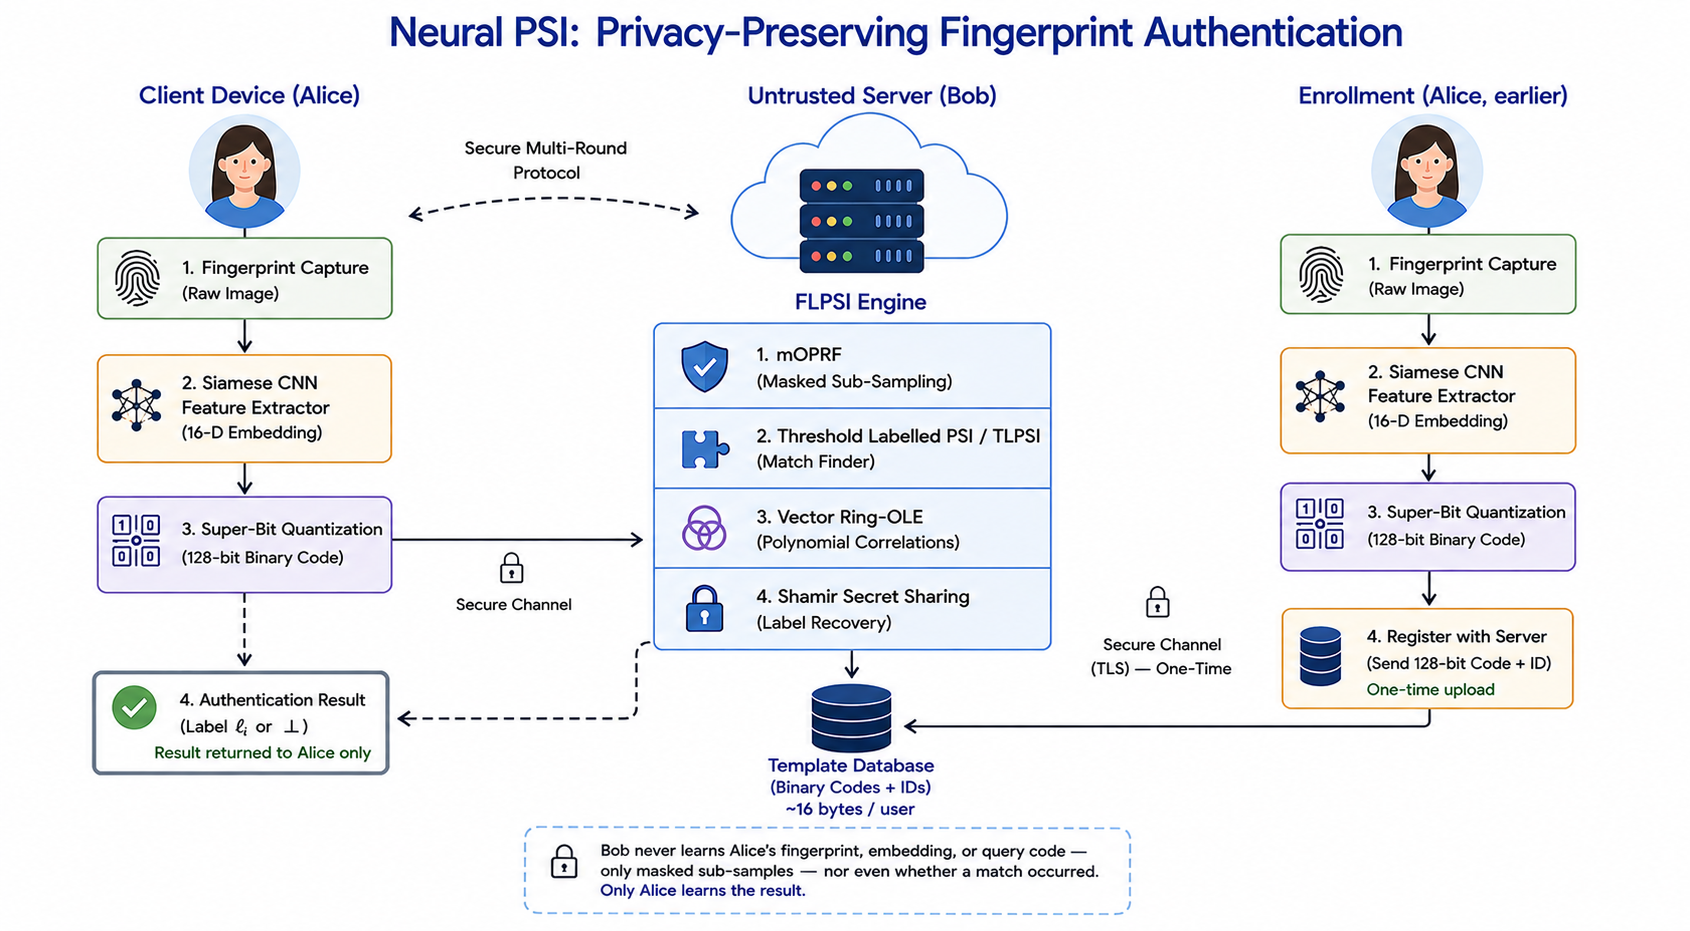
\includegraphics[width=0.78\linewidth]{neuralpsi-architecture.png}
\caption{The three stages. The CNN and quantiser run on the client in plaintext; only the
protocol messages leave the device. The server stores 16-byte codes and labels, with no key
material beyond a PRF key and no homomorphic layer.}
\label{fig:arch}
\end{figure}

NeuralPSI has three stages (Figure~\ref{fig:arch}). A Siamese CNN maps a capture to
$\mathbf{e} \in \mathbb{R}^{16}$; a public, training-free quantiser maps $\mathbf{e}$ to
$\xt \in \{0,1\}^{128}$; and FLPSI matches $\xt$ against the enrolled codes and returns the label
of any match. Stages one and two run entirely on the client. The server's entire per-user state
is a 16-byte code and a label.

The consequences of removing the homomorphic layer are immediate: server-side templates drop from
1.67\,KB to 16\,B, the 117\,MB Galois key disappears, and matching cost is linear in $N$ with no
slot-packing ceiling. What the composition costs is the subject of \S\ref{sec:params}.

\subsection{The quantisation bridge}
\label{sec:quantiser}

Replacing homomorphic matching with FLPSI creates a representation mismatch that nothing
downstream can paper over. The extractor emits a 16-dimensional real embedding whose natural
similarity is cosine; FLPSI matches fixed-length binary strings under Hamming distance with a
sub-sampling threshold. The bridge between them must satisfy four constraints at once, and most
off-the-shelf hashing schemes violate at least one:
(i)~\emph{similarity preservation} --- Hamming distance must track identity;
(ii)~\emph{fixed binary format} --- exactly $d = 128$ native Hamming bits;
(iii)~\emph{an FLPSI-friendly error profile} --- because the matcher sub-samples bit positions,
the bits must be balanced and the per-bit errors close enough to exchangeable that the
protocol's error analysis holds; and
(iv)~\emph{a public, cheap map} --- published alongside the model, costing one matrix multiply.

Constraint~(iii) is usually asserted. We measure it in \S\ref{sec:params}, and the result is
mixed: the bits are well balanced and the hypergeometric sub-sample model survives, but the bits
are strongly dependent and the resulting Hamming distribution is not the one the analysis
assumes.

Our quantiser is a fixed, public, \emph{affine-then-sign} map with no learned non-linearity, in
three stages. \textbf{(1)~Centre:} $\mathbf{e}_0 = \mathbf{e} - \boldsymbol{\mu}$, with
$\boldsymbol{\mu}$ the population mean on a calibration split disjoint from all evaluation
identities; L2-normalised features occupy a spherical cap rather than the full sphere, so
thresholding at the origin would give badly unbalanced bits. \textbf{(2)~Super-Bit projection:}
$\mathbf{z} = \mathbf{P}\mathbf{e}_0$ with $\mathbf{P} \in \mathbb{R}^{128 \times 16}$ built from
8 stacked $16 \times 16$ Gaussian blocks, each orthonormalised within the block by
Gram--Schmidt, all generated from one published seed. \textbf{(3)~Balanced sign:}
$\tilde{x}_k = \mathbf{1}[z_k > \tau_k]$ with $\tau_k$ the per-bit median on the calibration
split. At inference the three stages collapse to
\begin{equation}
\xt = \mathbf{1}\bigl[\mathbf{P}(\mathbf{e} - \boldsymbol{\mu}) > \boldsymbol{\tau}\bigr],
\end{equation}
and the public constants $(\mathbf{P}, \boldsymbol{\mu}, \boldsymbol{\tau})$ ship beside the
model as batch-normalisation statistics would.

Similarity is preserved by the random-hyperplane identity: for unit vectors at angle $\vartheta$,
\begin{equation}
\label{eq:lsh}
\frac{\mathbb{E}\bigl[\mathrm{Hamming}(\xt_1, \xt_2)\bigr]}{d}
 = \frac{\vartheta}{\pi}
 = \frac{1}{\pi}\arccos\bigl(\langle \hat{\mathbf{e}}_1, \hat{\mathbf{e}}_2\rangle\bigr),
\end{equation}
mapping genuine pairs to small Hamming distance and impostor pairs to large --- exactly the
quantity FLPSI thresholds. We use Super-Bit rather than plain SimHash because block
orthonormalisation leaves~\eqref{eq:lsh} unbiased while strictly lowering its variance at the
acute angles that separate genuine from impostor pairs, at the same 128 bits and no extra cost.

An optional fourth stage --- rescaling dimensions by $\mathrm{diag}(\sqrt{|\mathbf{w}_1|})$, the
head's final-layer weights, so Hamming distance tracks the learned accept metric rather than raw
cosine --- helps an under-trained embedding and \emph{hurts} a well-trained one
(\S\ref{sec:eval}). Our recommended configuration omits it.

\paragraph{The map is not a privacy mechanism.}
It is tempting to argue that publishing $\mathbf{P}$ is harmless because recovering $\mathbf{e}$
from $\xt$ means inverting an underdetermined system. \emph{This reasoning is backwards and we
flag it explicitly.} The map applies 128 sign measurements to a 16-dimensional vector --- an
\emph{over}-determined, roughly $8\times$ oversampled system --- and one-bit compressed
sensing~\cite{PlanVershynin13,JacquesEtAl13} recovers the \emph{direction} of $\mathbf{e}$ from
public $\mathbf{P}$ and $\xt$ to within an angular error that shrinks with the oversampling
ratio. \S\ref{sec:atrest} puts the number at $2.9$--$7.2^\circ$ against a genuine intra-class
spread of $11.7^\circ$, so the recovered direction re-quantises inside the accept region.

The sign map is therefore \emph{not} one-way and must not be relied on as one. Biometric privacy
rests entirely on the protocol: the server is the mOPRF \emph{sender} and never sees $\xt$ or any
plaintext sub-sample of it, so its view is simulatable from its own input (\S\ref{sec:security}).
The bridge's responsibility is accuracy and format; secrecy is discharged by the protocol, and
confidentiality \emph{at rest} is discharged by neither (\S\ref{sec:atrest}).

\subsection{Registration}

A user enrols by capturing a print, computing $\yt_u$ locally with the same public constants, and
sending $(\yt_u, \ell_u)$ over an authenticated channel. Enrolment must be authenticated: an
attacker able to enrol chosen codes can probe the code space directly (\S\ref{sec:attacks}). The
label $\ell_u$ is a 256-bit secret, and the server additionally stores the verifier
$V_u = \mathsf{H}(\ell_u)$ used by the credential step of \S\ref{sec:whoauth}.

\subsection{Authentication}

\begin{enumerate}\itemsep2pt
\item The client captures a print and computes $\xt$ locally. The server sends a fresh nonce
      $\nu$, folded into the first flow at no extra round.
\item Client and server run the masked OPRF over the $T$ public masks; for each mask the client
      learns a value determined by its own sub-sample and the server's key, and the server learns
      nothing about $\xt$.
\item For every record $i$ the server encodes Shamir shares of $\ell_i$ against the PRF images of
      $\yt_i$'s sub-samples and delivers them through the vector ring-OLE encoding. This is one
      batched pass, not $N$ independent instances --- all records share the client's receiver
      polynomial, which makes the batching cheap and is what \S\ref{sec:hybrids} must account for.
\item The client reconstructs $\ell_i$ for any record on which at least $\theta$ sub-samples
      collided, and replies $\sigma = \mathsf{HMAC}_{\ell_i}(\nu \,\|\, \mathsf{sid})$.
\item The server verifies $\sigma$ against its stored verifiers and grants the session.
\end{enumerate}

Steps 1--4 realise $\Fnpsi$; step 5 turns a private lookup into an authentication, which the
functionality alone does not provide (\S\ref{sec:whoauth}). The nonce and session identifier are
what stop $\sigma$ being replayable: $\ell$ is a long-lived per-user secret, so without them one
intercepted transcript would be a permanent credential.

% =============================================================================
%  Parameter selection and error analysis.
%  SHARED: \input by both paper.tex (as Section 5) and technical-report.tex,
%  so the two documents cannot report different numbers.
% =============================================================================
\section{Parameter Selection and Error Analysis}
\label{sec:params}

The FLPSI layer is parameterised by the code length $d$, the number of sub-samples $T$, the
sub-sample width $w$, and the acceptance threshold $\theta$. This section derives the error
rates those parameters induce, and shows that the published choice
$(d,T,w,\theta) = (128, 64, 14, 2)$ is wrong by three orders of magnitude on real codes --- not
because the arithmetic is wrong, but because the distribution it assumes is.

\subsection{The accept model}

A sub-sample selects $w$ of the $d$ positions uniformly at random and collides when the two
codes agree on all of them. Writing $H = \|\xt \oplus \yt_i\|_1$ for the Hamming distance, the
per-sub-sample collision probability and the acceptance probability are
\begin{equation}
\label{eq:accept}
q(H) \;=\; \frac{\binom{d-H}{w}}{\binom{d}{w}},
\qquad
\Pr[\text{accept} \mid H] \;=\; \Pr\bigl[\mathrm{Binomial}(T, q(H)) \ge \theta\bigr].
\end{equation}
Acceptance depends on the pair \emph{only through $H$} --- not on which positions differ ---
because the mask is a uniformly random set. Consequently the false-accept and false-reject
rates are exact functionals of the two Hamming histograms,
\begin{equation}
\label{eq:rates}
\mathrm{FAR} = \sum_{H} P_{\mathrm{imp}}(H)\,\Pr[\text{accept}\mid H],
\qquad
\mathrm{FRR} = 1 - \sum_{H} P_{\mathrm{gen}}(H)\,\Pr[\text{accept}\mid H],
\end{equation}
with no Monte-Carlo error. Every number below is computed from~\eqref{eq:rates} over 1,200
held-out identities: 1,200 genuine and 2,877,600 impostor pairs.

\paragraph{Validating the model before using it.}
Equation~\eqref{eq:accept} assumes the $d$ positions are exchangeable, and Super-Bit's advantage
comes precisely from making bits \emph{dependent}, so this needs testing. Measuring $\hat q(H)$
on real code pairs (200 sub-sample draws per pair, $w=14$) gives $\hat q(H)/q(H)$ with
\textbf{median $1.002$, range $[0.919, 1.099]$} over $H \in [5,40]$. Bit dependence is real ---
mean inter-bit $|\rho| = 0.254$, and the correlation matrix has participation ratio $9.84$, so
the 128 bits behave like about ten independent decisions --- but it manifests in the distribution
\emph{of} $H$, not in $\Pr[\text{accept}\mid H]$. That isolates the defect to one place and
licenses~\eqref{eq:rates}.

\subsection{The codes are balanced but not uniform}

The parameters were selected under a model in which impostor codes are uniform, giving
$H \sim \mathrm{Binomial}(128, \tfrac12)$ with $\sigma = 5.66$. Table~\ref{tab:dist} compares
that model against measurement.

\begin{table}[htbp]
\centering
\caption{Impostor Hamming distribution: assumed versus measured over 2,877,600 held-out pairs.
The mean is exactly as predicted; nothing else is.}
\label{tab:dist}
\small
\begin{tabular}{@{}lrr@{}}
\toprule
& uniform model & measured \\
\midrule
mean $H$              & 64.0 & \textbf{64.0} \\
standard deviation    & 5.66 & \textbf{20.22} \\
minimum observed $H$  & --- (never below $\approx$40) & \textbf{0} \\
\midrule
genuine mean $H$ & --- & 8.3 (sd 5.67, max 34) \\
\bottomrule
\end{tabular}
\end{table}

The mean is \emph{exactly} right, because the quantiser's median-thresholding step balances
every bit (measured balance $\in [0.466, 0.540]$). \textbf{No first-moment check can detect this
failure}: a sanity test verifying that impostor codes ``look like coin flips on average'' passes
cleanly. The discrepancy is entirely in the second moment and the tail, where $\sigma$ is
$3.6\times$ larger than assumed.

The cause is structural rather than a defect of this particular bridge. A 128-bit Super-Bit code
is 128 projections of a 16-dimensional embedding, so it carries roughly 16 real degrees of
freedom. The bridge is \emph{faithful} --- $\mathbb{E}[H]/d = \arccos(\text{cos-sim})/\pi$ holds
--- and that faithfulness is the problem: it transmits the embedding's angular distribution
intact, including the fact that some fingers genuinely resemble one another. We expect any LSH
bridge over a learned low-dimensional embedding to behave the same way.

\begin{figure}[htbp]
\centering
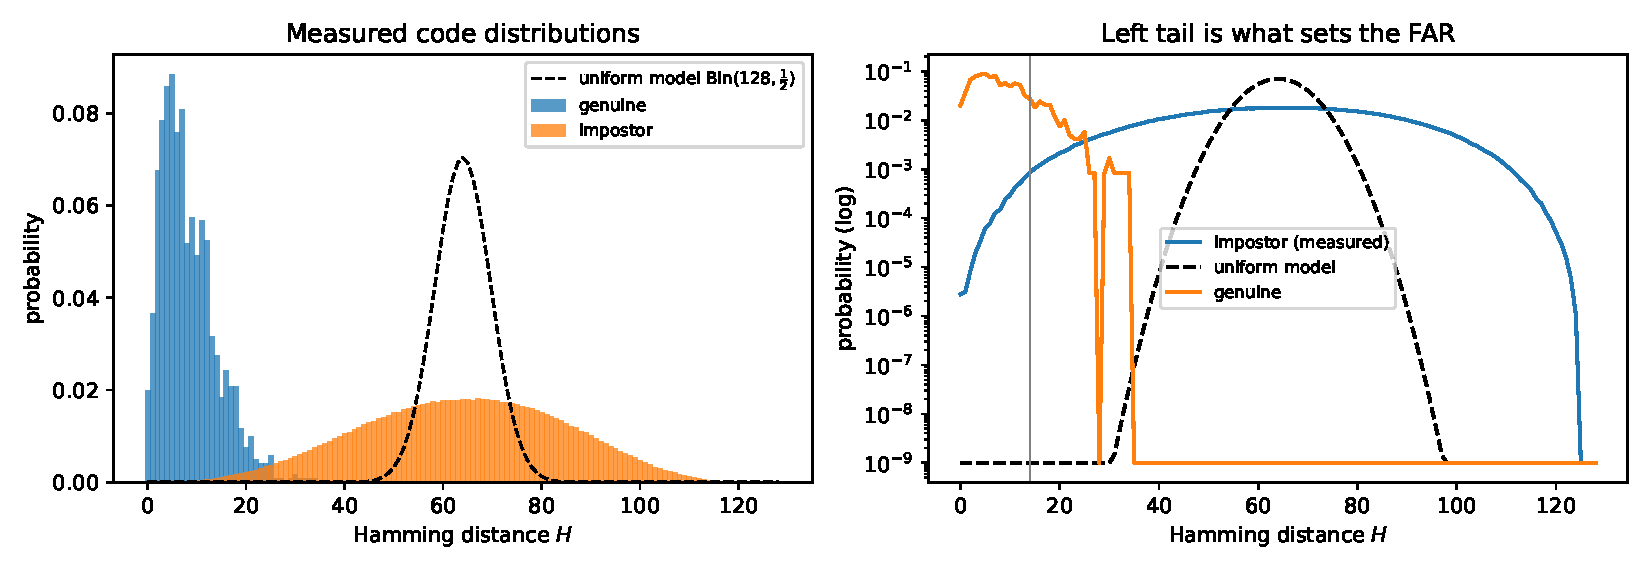
\includegraphics[width=0.82\linewidth]{hamming-histograms.pdf}
\caption{Measured genuine and impostor Hamming distributions against the uniform model
(dashed). Left: linear scale, where the impostor mean sits exactly at $d/2$. Right: log scale,
where the left tail --- the part that sets the false-accept rate --- is several orders of
magnitude heavier than assumed.}
\label{fig:hist}
\end{figure}

\subsection{The consequence for the published operating point}

At $(w,\theta) = (14,2)$ with error-free sub-samples, evaluating~\eqref{eq:rates} against the
uniform model reproduces the published per-record false-accept rate of $2.954\times10^{-5}$
exactly, and $q(8) = \binom{120}{14}/\binom{128}{14} = 0.38493266$ matches the published
constant to all quoted digits. The arithmetic is sound. Against the \emph{measured}
distribution the same expressions give
\begin{center}\small
\begin{tabular}{@{}lrrr@{}}
\toprule
& uniform model & measured & ratio \\
\midrule
per-record FAR & $2.954\times10^{-5}$ & $\mathbf{4.578\times10^{-2}}$ & $\mathbf{1{,}550\times}$ \\
FRR & --- & $9.61\times10^{-3}$ & --- \\
\bottomrule
\end{tabular}
\end{center}

A per-record rate is not a security boundary. A $1{:}N$ identification query is tested against
every enrolled record, so what an attacker faces is
$\mathrm{FAR}_{\text{query}} = 1-(1-\mathrm{FAR})^{N}$ (Figure~\ref{fig:farn}):

\begin{center}\small
\begin{tabular}{@{}lrrrrrr@{}}
\toprule
$N$ & 1 & 10 & 100 & 1{,}000 & 5{,}000 & $10^{4}$ \\
\midrule
$\mathrm{FAR}_{\text{query}}$, published point & 0.046 & 0.374 & \textbf{0.991} & 1.000 & 1.000 & 1.000 \\
$\mathrm{FAR}_{\text{query}}$, collision floor & --- & --- & 0.0003 & 0.0028 & \textbf{0.0138} & 0.0274 \\
\bottomrule
\end{tabular}
\end{center}

FRR is $0.96\%$ throughout. \textbf{The published parameters describe a verification $(1{:}1)$
system, not an identification system}: at $N=1$ a $4.6\%$ false-accept rate is poor but coherent,
and by $N=100$ the query-level rate already exceeds $50\%$. The second row is the irreducible
floor derived in \S\ref{sec:floor}, which no parameter choice can go below.

\begin{figure}[htbp]
\centering
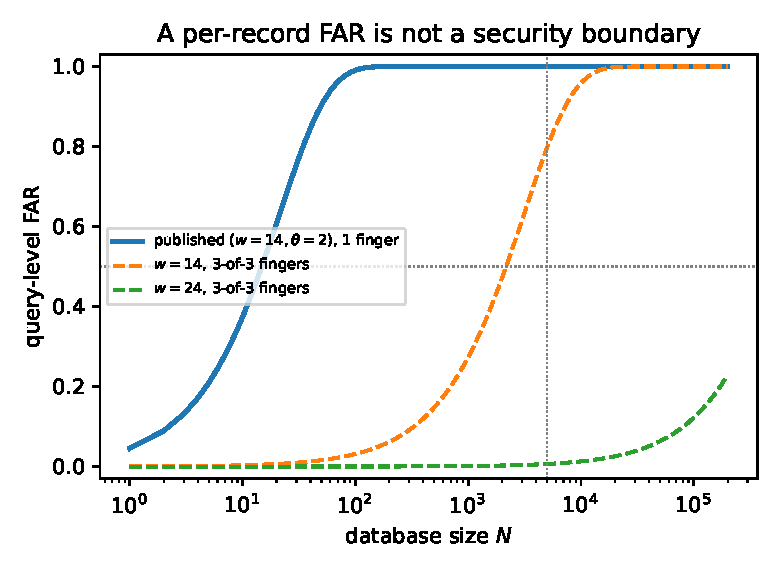
\includegraphics[width=0.52\linewidth]{far-vs-dbsize.pdf}
\caption{Query-level false-accept rate against database size. The published single-finger point
crosses $50\%$ at $N \approx 100$. Multi-finger fusion moves the curve by orders of magnitude;
retuning does not.}
\label{fig:farn}
\end{figure}

\subsection{Retuning does not repair it}

We swept 6,848 combinations of $w \in \{8,\dots,64\}$, $t \in \{0,\dots,8\}$ and
$\theta \in \{1,\dots,64\}$, keeping only points whose FAR estimate is supported by the
histogram (less than half the FAR mass drawn from bins holding fewer than ten observed pairs).
Taking the lowest-FRR point that meets each query-level target at $N = 5{,}000$:

only one target is reachable at all. A query-level rate of $10^{-1}$ is met by
$(w,t,\theta) = (56,1,40)$ --- at an FRR of \textbf{84.8\%} --- and $10^{-2}$, $10^{-3}$ and
$10^{-4}$ are unreachable by any point in the sweep with usable histogram support. The only
setting that reaches even a $10\%$ query FAR rejects $85\%$ of legitimate users. The
suggestion that $\theta$ should grow as $\Theta(\log N)$ to hold the query-level rate constant
is directionally right and quantitatively insufficient, for the reason we give next.

\subsection{An irreducible collision floor}
\label{sec:floor}

\textbf{8 of the 2,877,600 impostor pairs have Hamming distance exactly zero} --- distinct
fingers producing \emph{identical} 128-bit codes. The collision rate is
\begin{equation}
p_0 = 2.78\times10^{-6}, \qquad \text{exact Poisson 95\% CI } [1.20\times10^{-6},\, 5.48\times10^{-6}].
\end{equation}
Since $q(0) = 1$, every sub-sample collides and $\Pr[\text{accept}\mid H{=}0] = 1$ for
\emph{every} $(w, t, \theta)$. Therefore $p_0$ is a \textbf{hard lower bound on the per-record
false-accept rate of any FLPSI parameterisation over these codes}, and it propagates to the query
level as tabulated above. This is precisely why the ladder above becomes unreachable below $10^{-2}$: at $N = 5{,}000$ the
floor alone is $1.4\%$, independent of $\theta$. The near tail is dense as well --- $1.03\times
10^{-3}$ of impostor pairs lie at $H \le 10$, and $2.80\times10^{-2}$ at $H \le 25$, which is the
99th percentile of the \emph{genuine} distribution. The two distributions genuinely overlap; the
protocol is being asked to separate things that are not separable.

\textbf{The bound is a property of the code, not of the protocol.} It moves only by producing
better codes, and it is cheap for any future system to report: count $H = 0$ pairs on a held-out
set. We recommend it as a standard diagnostic for fuzzy-PSI-over-learned-codes constructions.

\subsection{Multi-finger fusion is the lever that works}

Each finger is a separate enrolment, so $k$-of-$K$ fusion multiplies evidence instead of trading
FAR against FRR along one curve --- and it is the only mechanism here that can beat the
single-finger floor, since $k$ fingers must collide simultaneously. We measure it over 201
held-out subjects contributing at least three fingers each, computing a Poisson-binomial over
the real per-finger accept probabilities, so any correlation between one person's own fingers is
carried by the data rather than assumed away.

\begin{table}[htbp]
\centering
\caption{Measured $k$-of-$K$ fusion at $N = 5{,}000$, over 201 held-out subjects.}
\label{tab:fusion}
\small
\begin{tabular}{@{}llrrr@{}}
\toprule
parameters & rule & per-record FAR & $\mathrm{FAR}_{\text{query}}$ & FRR \\
\midrule
$w{=}14$, $\theta{=}2$ & 1-of-3 & $1.31\times10^{-1}$ & 1.000 & 0.000 \\
$w{=}14$, $\theta{=}2$ & 2-of-3 & $8.73\times10^{-3}$ & 1.000 & 0.001 \\
$w{=}14$, $\theta{=}2$ & 3-of-3 & $3.19\times10^{-4}$ & 0.797 & 0.026 \\
$w{=}24$, $\theta{=}2$ & 1-of-3 & $1.95\times10^{-2}$ & 1.000 & 0.002 \\
$w{=}24$, $\theta{=}2$ & 2-of-3 & $2.45\times10^{-4}$ & 0.707 & 0.033 \\
\textbf{$w{=}24$, $\theta{=}2$} & \textbf{3-of-3} & $\mathbf{1.30\times10^{-6}}$ &
  \textbf{0.0065} & \textbf{0.281} \\
\bottomrule
\end{tabular}
\end{table}

Fusion buys four orders of magnitude on the per-record rate, far more than any single-finger
retuning achieves. It is still not sufficient on its own: the best measured configuration costs
a $28\%$ false-reject rate. The honest summary is that \textbf{at $N = 5{,}000$ with a
16-dimensional embedding, no configuration of this protocol is simultaneously secure and
usable}.

\paragraph{What this means for parameter selection.} Report FLPSI biometric parameters as a
verification operating point unless the query-level rate at the target $N$ is stated; fit them to
the \emph{measured} code distribution, since the uniform assumption errs by $1{,}550\times$ here
and fails silently; and publish the collision floor of \S\ref{sec:floor}, which bounds every
parameter choice and costs one pass over a held-out set. The remedy is more evidence, not a
different threshold, and the binding constraint is the embedding dimension --- sixteen dimensions
cannot separate 5,000 identities at cryptographic error rates.

% =============================================================================
%  Security analysis.  Slots into the restructured paper as Section 6 (2.5 pp).
%  The long-form hybrid sequence lives in sections/appendix-hybrids.tex.
% =============================================================================
\section{Security Analysis}
\label{sec:security}

We work in the semi-honest model with static corruptions. Throughout, $\lambda$ is the
computational security parameter, $\kappa$ the statistical one, $\mathbb{F}$ a field with
$|\mathbb{F}| \ge 2^{\kappa + \log N}$, and $\mathsf{negl}$ an unspecified negligible
function. Section~\ref{sec:atrest} then steps outside that model, because the most
serious weakness we identify is not a protocol weakness at all.

\subsection{The functionality}
\label{sec:functionality}

Prior work in this line proves security for \emph{one} client set against \emph{one}
labelled server set. NeuralPSI runs $N$ record instances sharing a receiver polynomial
and a PRF key, so the composite object needs to be named before anything can be proved
about it.

\begin{figure}[htbp]
\fbox{\parbox{0.97\linewidth}{
\textbf{Functionality} $\mathcal{F}_{\mathsf{NeuralPSI}}^{d,T,w,\theta}$\\[2pt]
\textbf{Parties.} A client $\mathsf{C}$ and a server $\mathsf{S}$.\\
\textbf{Parameters.} Code length $d$, sub-sample count $T$, sub-sample width $w$,
acceptance threshold $\theta$, and a public mask family
$M = \{m_j\}_{j\in[T]}$, $m_j \in \{0,1\}^d$, $\|m_j\|_1 = w$.\\[3pt]
\textbf{Inputs.} $\mathsf{C}$ inputs $\tilde{\mathbf{x}} \in \{0,1\}^d$.
$\mathsf{S}$ inputs a database $D = \{(\tilde{\mathbf{y}}_i, \ell_i)\}_{i\in[N]}$ with
$\tilde{\mathbf{y}}_i \in \{0,1\}^d$ and labels $\ell_i \in \mathbb{F}$.\\[3pt]
\textbf{Computation.} For each $i \in [N]$ let
\[
S_i \;=\; \bigl\{\, j \in [T] \;:\; \tilde{\mathbf{x}} \wedge m_j
   \;=\; \tilde{\mathbf{y}}_i \wedge m_j \,\bigr\},
\qquad
\mathsf{acc}(i) \;=\; \bigl[\,|S_i| \ge \theta\,\bigr].
\]
\textbf{Outputs.} $\mathsf{C}$ receives $\mathsf{out} =
\{\,(i, \ell_i) : \mathsf{acc}(i)\,\}$; $\mathsf{S}$ receives $\bot$.
}}
\caption{The composite functionality. Note that the output is a \emph{set}: the scan runs
over all $N$ records and more than one may satisfy the predicate. This differs from the
single-match phrasing used in earlier drafts of this work, and the difference is
observable --- $|\mathsf{out}| > 1$ occurs at a rate we measure in
Section~\ref{sec:params}.}
\label{fig:functionality}
\end{figure}

Two features of Figure~\ref{fig:functionality} deserve emphasis. First, acceptance is a
deterministic function of $\tilde{\mathbf{x}}$, $\tilde{\mathbf{y}}_i$ and the public mask
family, so it depends on the pair only through which positions differ; because the masks
are drawn uniformly it depends in distribution only on the Hamming weight
$H = \|\tilde{\mathbf{x}} \oplus \tilde{\mathbf{y}}_i\|_1$. Every error rate in
Section~\ref{sec:params} follows from that observation. Second, the functionality says
nothing about \emph{authentication}: no party other than $\mathsf{C}$ learns anything, so
a relying party cannot act on the result. We return to this in
Section~\ref{sec:whoauth}.

\paragraph{The masks are public.} We fix this now because the leakage analysis depends on
it. Taking $M$ public is the conservative reading: it gives the adversary strictly more
than a server-private mask family would, and our claims hold under it. Making $M$
server-private would shrink $\mathcal{L}_{\mathsf{C}}$ below, but the protocol as
constructed delivers the collision pattern to the client, so a private $M$ would require a
structural change rather than a parameter choice.

\subsection{The leakage function}
\label{sec:leakage}

$\mathcal{F}_{\mathsf{NeuralPSI}}$ is what we would like to realise. What the protocol
realises is $\mathcal{F}_{\mathsf{NeuralPSI}}$ \emph{augmented with leakage}:
\begin{align}
\mathcal{L}_{\mathsf{C}}(\tilde{\mathbf{x}}, D) &=
  \Bigl(\;N,\;\; \bigl\{\,(i, S_i) \;:\; |S_i| \ge \theta \,\bigr\} \;\Bigr),
  \label{eq:leakC}\\[2pt]
\mathcal{L}_{\mathsf{S}}(\tilde{\mathbf{x}}, D) &= \bot .
  \label{eq:leakS}
\end{align}

Equation~\eqref{eq:leakC} is strictly more than ``the identity of the matched record''.
The client learns \emph{which} sub-samples collided, and since $M$ is public, each
$j \in S_i$ pins $w$ known positions of $\tilde{\mathbf{y}}_i$ to known values. The client
also learns $N$, the number of records tested. We quantify the consequences in
Section~\ref{sec:attacks}; the short version is that $\mathcal{L}_{\mathsf{C}}$ is enough
to reconstruct a matched record outright.

\subsection{Security theorem}

\begin{theorem}[Semi-honest security]
\label{thm:main}
Let $F$ be a PRF, and instantiate the sub-protocols with a masked OPRF
$\Pi_{\mathsf{mOPRF}}$ and a vector ring-OLE $\Pi_{\mathsf{VROLE}}$, each semi-honest
secure. Then the NeuralPSI protocol of Section~\ref{sec:design} securely realises
$\mathcal{F}_{\mathsf{NeuralPSI}}^{d,T,w,\theta}$ with leakage
$(\mathcal{L}_{\mathsf{C}}, \mathcal{L}_{\mathsf{S}})$ against a semi-honest adversary
statically corrupting one party. Concretely, for every such adversary $\mathcal{A}$ there
is a simulator whose output is distinguishable from $\mathcal{A}$'s view with advantage at
most
\begin{equation}
\label{eq:bound}
\varepsilon \;\le\;
   \varepsilon_{\mathsf{mOPRF}}
 + \varepsilon_{\mathsf{VROLE}}
 + \varepsilon_{\mathsf{LPN}}
 + \underbrace{\varepsilon_{F}\bigl(q + T\!\cdot\!2^{w}\bigr)}_{\text{PRF, extended domain}}
 + \underbrace{\frac{N(2T+1)}{|\mathbb{F}|}}_{\text{statistical}} ,
\end{equation}
where $q$ is the adversary's own query count.
\end{theorem}

Two terms in~\eqref{eq:bound} are easy to omit and both matter. The PRF term is charged
for $T \cdot 2^{w}$ extra oracle queries, not $q$ alone: each mask restricts the PRF input
to a domain of size $2^{w} = 2^{14}$, so the full input table has only
$T \cdot 2^{w} = 2^{20}$ entries and the reduction must budget for enumerating it. The
statistical term is the price of the polynomial masking step (hybrid $\mathsf{H}_4$
below) and is the reason $|\mathbb{F}|$ must be chosen with $N$ in view; we report the
concrete field size in Section~\ref{sec:eval}.

Both simulators are constructed in Appendix~\ref{app:hybrids}. The corrupt-client simulator
takes $\xt$ and $(\mathsf{out}, \mathcal{L}_{\mathsf{C}})$ and produces the mOPRF outputs, the
sender-side silent-VOLE transcript and the polynomials $\{\hat z_i\}$, sampling uniformly at every
point not pinned by $\mathcal{L}_{\mathsf{C}}$. The corrupt-server simulator has only the
transcript to produce, since the server outputs $\bot$; its one input-dependent message is
$\Delta U = \Delta u(X)$. Worth stating precisely, because the natural argument is slightly wrong:
$\Delta U$ is \emph{not} uniform on $\mathbb{F}^{2T+1}$ but lies in the $(T{+}1)$-dimensional image
of the degree-$\le T$ evaluation map, so the simulator samples a uniform polynomial of degree
$\le T$ and outputs its evaluation vector. Since $u'_0$ is uniform, $u_0 - u'_0$ is uniform
\emph{in that subspace} and the indistinguishability is statistical, not computational.

\subsection{Hybrids}
\label{sec:hybrids}

$\mathsf{H}_0$ is the real execution. $\mathsf{H}_1$ replaces $\Pi_{\mathsf{mOPRF}}$ by
$\mathcal{F}_{\mathsf{mOPRF}}^{T}$ (semi-honest mOPRF security); $\mathsf{H}_2$ replaces $F_k$ by
a random function (PRF security, charged at $q + T\cdot2^{w}$ queries as above); $\mathsf{H}_3$
replaces $\Pi_{\mathsf{VROLE}}$ by $\mathcal{F}_{\mathsf{VROLE}}$ (base-VOLE security and LPN).

$\mathsf{H}_4$ is the load-bearing \emph{statistical} step, and is the one most easily left
unstated: for every non-colliding point $x_j$ it replaces
$v_1(x_j) = f(x_j) + \bigl(\prod_i (x_j - \yt_i)\bigr)\cdot R(x_j)$ by a uniform element of
$\mathbb{F}$. This holds because $R$ is uniform of degree $\le T$ and the evaluation map on any
set of at most $T+1$ points is a bijection onto $\mathbb{F}^{T+1}$, so the masking terms are
jointly uniform --- \emph{provided}
\begin{equation}
\label{eq:h4}
\bigl|\{\, j \in [T] : j \notin S_i \,\}\bigr| \;\le\; \deg R + 1 \;=\; T+1,
\end{equation}
which holds unconditionally here since $|[T]| = T$, but is a design constraint rather than an
accident. Over $N$ records and $2T+1$ points the union bound gives the $N(2T+1)/|\mathbb{F}|$
term in~\eqref{eq:bound}. Finally $\mathsf{H}_5$ replaces $\ell'_i = F_k(\ell_i)$ by uniform
elements (immediate from $\mathsf{H}_2$), and $\mathsf{H}_6 = \mathsf{Sim}_{\mathsf{C}}$ is
identical by inspection.

\paragraph{Why $N$ instances do not compose for free.}
The step that a citation cannot discharge is the reuse across records. All $N$ record
instances share one receiver polynomial $u_0$ --- that sharing is precisely what makes the
vector ring-OLE batching asymmetric and cheap --- and one PRF key $k$, across all records
\emph{and} all sessions. Hybrids $\mathsf{H}_2$ and $\mathsf{H}_4$ are therefore stated
over the whole database rather than per record: $\mathsf{H}_2$ replaces the single shared
$F_k$ once, which is why its cost appears once rather than $N$ times, and $\mathsf{H}_4$
is applied simultaneously at all $N(2T+1)$ points with the union bound
in~\eqref{eq:bound}. Constraint~\eqref{eq:h4} must hold for every record at once; it does,
but only because $\deg R \ge T$, which is a design requirement rather than an accident and
is easy to violate when tuning $T$ downward for communication.

The long-form hybrids, with the distinguisher reductions written out, are in
Appendix~\ref{app:hybrids}.

\subsection{The stored template is a bearer credential}
\label{sec:atrest}

Theorem~\ref{thm:main} covers the protocol and says nothing about data at rest, which is where
this design is weakest --- strictly weaker than the homomorphic baseline, whose stored feature
vectors are encrypted under a key the server never holds.

The server stores $(\yt_i, \ell_i)$ in the clear. An adversary who reads $\yt_i$ and submits it
as a query obtains $H = 0$, hence $|S_i| = T$ and acceptance with probability $1$. \emph{No
inversion is required}: the stored code \emph{is} a working credential, so a database breach is
immediate and total impersonation of every enrolled user.

Inversion is an additional problem. The quantiser is over-determined --- 128 hyperplanes cut
$\mathbb{S}^{15}$ into $2\sum_{k<16}\binom{127}{k} \approx 2^{64.5}$ cells --- so it is not
one-way in any useful sense. Its intrinsic angular resolution is
$\text{cells}^{-1/15} \approx 2.9^\circ$, and the standard one-bit compressed-sensing heuristic
$k/m = 16/128$ gives $7.2^\circ$, against a measured genuine intra-class spread of
$\pi\cdot 8.3/128 = 11.7^\circ$. Reconstruction is thus $1.6$--$4\times$ \emph{tighter} than
genuine variation: the recovered direction re-quantises inside the accept region and transfers
to any system using the same extractor.

\begin{table}[htbp]
\centering
\caption{The stored template against ISO/IEC 24745~\cite{ISO24745}. NeuralPSI as
specified fails all three requirements.}
\label{tab:iso24745}
\small
\begin{tabular}{@{}p{0.19\linewidth}p{0.10\linewidth}p{0.62\linewidth}@{}}
\toprule
\textbf{Requirement} & \textbf{Status} & \textbf{Why} \\
\midrule
Irreversibility & fails & Twice: direct replay of the stored code, and one-bit
compressed-sensing recovery of the embedding direction to $2.9$--$7.2^\circ$. \\
Unlinkability & fails & $(P, \mu, \tau)$ and the projection seed are public and fixed, so
one finger yields the same 128-bit code in every deployment and codes are directly
Hamming-comparable across databases. There is no diversification parameter. \\
Renewability & fails & A second independent code cannot be issued from the same finger.
This is the requirement the application most needs, since a compromised fingerprint
cannot be reissued. \\
\bottomrule
\end{tabular}
\end{table}

\paragraph{Mitigations, and what they actually buy.}
\emph{(i) A client-side per-enrolment XOR mask}: the device holds $r_u \in \{0,1\}^{d}$ and the
server stores $\yt \oplus r_u$. XOR preserves Hamming distance exactly, so \textbf{accuracy is
unchanged} --- every number in \S\ref{sec:eval} carries over --- and 16 bytes of client state
buys unlinkability and renewability. It does \emph{not} stop replay of a stolen record.
\emph{(ii) Envelope encryption at rest}, key in an HSM, decrypting to memory for the scan:
unglamorous, orthogonal to the protocol, sound in the semi-honest model, and what we would
deploy. \emph{(iii)} We explicitly reject one tempting option --- storing the mOPRF images
$\{F_k(\yt_i \wedge m_j)\}_j$ instead of the code. It is keyed and locality-preserving and the
server computes those values anyway, but the per-mask domain is only $2^{w} = 2^{14}$, so anyone
who can evaluate $F_k$ inverts each image by exhaustive search; repairing it needs a per-record
salt that destroys the equality-preservation the protocol depends on.

Applying (i) and (ii) yields unlinkability and renewability. \textbf{Full at-rest
confidentiality against a compromised server remains out of scope}, and this posture is weaker
than the encrypted-template baseline's --- a limitation we state rather than resolve.

\subsection{Who is actually authenticated}
\label{sec:whoauth}

As specified, no relying party learns the outcome, so no session can be granted:
$\mathcal{F}_{\mathsf{NeuralPSI}}$ is a private identification lookup, not an authentication
protocol. The credential step of Section~\ref{sec:design} closes the gap for one MAC, one nonce
and 32 bytes, with the nonce and session id making $\sigma$ non-replayable --- without them one
intercepted transcript is a permanent credential, since $\ell$ is long-lived.

That step has a consequence for how Section~\ref{sec:params} should be read. A client cannot
forge $\sigma$ without $\ell_i$, so system security reduces to recovering \emph{some} $\ell_i$,
which is exactly the false-accept question. In a conventional matcher a false accept is one bad
login; here it hands the attacker a \textbf{permanent per-user credential}. \emph{The
false-accept rate is a credential-compromise rate}, which is why we treat it as a security
parameter rather than an accuracy metric.

\subsection{Attacks}
\label{sec:attacks}

\paragraph{(a) Impersonation without search.}
The parameters were chosen against an attacker submitting \emph{uniformly random} codes,
for which the per-record accept probability is $q_{\mathsf{rand}} = 2.954\times10^{-5}$.
But the cheapest attack is not to guess: it is to present one's own finger. Measured over
$2.88\times10^{6}$ held-out impostor pairs, the per-record accept probability for a
\emph{real but wrong} finger is $q_{\mathsf{bio}} = 4.578\times10^{-2}$ --- $1{,}550\times$
larger. Expected queries to impersonate somebody, $1/(1-(1-q)^N)$:

\begin{center}\small
\begin{tabular}{@{}lrrrr@{}}
\toprule
$N$ & $512$ & $5{,}000$ & $10^{5}$ & $10^{6}$ \\
\midrule
random code ($q_{\mathsf{rand}}$) & $67$ & $7$ & $1.05$ & $1$ \\
\textbf{zero-effort finger} ($q_{\mathsf{bio}}$) & $\mathbf{1}$ & $\mathbf{1}$ &
  $\mathbf{1}$ & $\mathbf{1}$ \\
\bottomrule
\end{tabular}
\end{center}

At every database size we measured, a single presentation of an unrelated finger
impersonates \emph{someone} with probability above $99\%$. Rate limiting does not
mitigate an attack that succeeds on the first attempt.

\paragraph{(b) Template recovery from the collision pattern.}
On any accept, $\mathcal{L}_{\mathsf{C}}$ gives the client $S_i$. With $\theta = 2$ the
client can enumerate all $\binom{64}{2} = 2{,}016$ candidate pairs, interpolate, and test,
so it learns $S_i$ exactly and cheaply. Because the masks are public, each $j \in S_i$
pins $w = 14$ known positions of $\tilde{\mathbf{y}}_i$. At $H \approx 8$ a genuine query
produces $T \cdot q(8) = 64 \times 0.38493 \approx 24.6$ collisions, covering
$24.6 \times 14 \approx 345$ position-slots over $128$ positions: \textbf{one successful
authentication determines the target record}. Recovering a \emph{chosen} user costs
$1/q_{\mathsf{bio}} \approx 22$ queries at the measured rate; recovering \emph{a} user's
full template at $N \ge 10^{5}$ costs one.

\paragraph{(c) The mOPRF dictionary.}
Each mask restricts the PRF domain to $2^{w} = 2^{14}$, and the entire table is
$T \cdot 2^{w} = 2^{20}$. A client learns one entry per mask per session, so a
coupon-collector argument gives roughly $1.1\times10^{4}$ sessions for $50\%$ coverage per
mask --- already sufficient, since 32 of 64 masks at 14 bits each over-determines a
128-bit code --- and about $1.7\times10^{5}$ sessions for full coverage. ``PRF-masked''
thus provides at most $w = 14$ bits of preimage resistance per sub-sample against a
querying client.

\paragraph{Required deployment controls.} Consequently: (i) rate limiting per account
\emph{and} per relying party, with the explicit admission that it does not mitigate (a) at
large $N$; (ii) authenticated enrolment, so an attacker cannot enrol chosen codes to probe
the space; (iii) per-epoch rotation of $k$ and of the mask family, at the stated
re-enrolment cost; (iv) sensor attestation as an explicit deployment assumption; and
(v) the nonce binding of Section~\ref{sec:whoauth}.

\paragraph{What we do not claim.} Malicious security --- cut-and-choose techniques exist for
related structure-aware PSI settings~\cite{GarimellaEtAl23}, but they target geometric-ball
rather than threshold predicates, so their overheads do not transfer and we do not estimate
them. At-rest confidentiality against a compromised server. That the quantiser is one-way: it
demonstrably is not, and no part of Theorem~\ref{thm:main} relies on it. And that the measured
false-accept rates are acceptable at the sizes we tested --- \S\ref{sec:params} shows they are
not, and why.

\section{Implementation and Evaluation}
\label{sec:eval}

\paragraph{Setup.} The extractor is trained on SOCOFing~\cite{Shehu18} (6,000 fingerprints, 600
subjects $\times$ 10 fingers) at $224\times224$, with an identity-disjoint split: 4,800 training
images and 1,200 held-out identities that appear in no training or calibration step. Enrolment
uses the \texttt{Real} captures and probes use the \texttt{Altered-*} sets. Confidence intervals
throughout are 95\% bootstrap over \emph{identities}, not pairs --- pairs sharing a finger are
not independent, and resampling pairs understates the interval. Hardware: RTX 4050 (6\,GB); the
FLPSI layer runs against a reference implementation of~\cite{BuiCong25} instrumented to count
protocol bytes.

\subsection{Accuracy}

\begin{table}[htbp]
\centering
\caption{EER with 95\% identity-level bootstrap intervals, at a matched bit budget. Collisions
count impostor pairs at $H = 0$ out of ${\approx}1.44$M.}
\label{tab:acc}
\small
\begin{tabular}{@{}lcccr@{}}
\toprule
Coder & Altered-Easy & Altered-Medium & Altered-Hard & $H{=}0$ \\
\midrule
Float embedding (ceiling) & 0.33\% & --- & --- & --- \\
\textbf{Super-Bit 128} & \textbf{1.88\%} [1.56, 2.20] & 4.48\% [3.90, 4.94] &
  7.04\% [6.31, 7.45] & \textbf{2} \\
ITQ 128 & 4.55\% [3.91, 5.31] & 7.11\% [6.39, 7.73] & 9.06\% [8.47, 9.75] & 517 \\
ITQ 16 & 6.13\% [5.54, 6.80] & 8.49\% [7.84, 9.19] & 11.58\% [10.56, 12.20] & 6{,}394 \\
Naive sign 16 & 10.12\% & --- & --- & --- \\
\bottomrule
\end{tabular}
\end{table}

Binarisation costs $+1.55$ percentage points of EER against the $0.33\%$ floating-point ceiling
(Table~\ref{tab:acc}). Two comparisons matter more than the headline.

First, \textbf{the bit budget}. Comparing a 128-bit Super-Bit code against a 16-bit ITQ code
would be a mismatch, so ITQ is fitted at 128 bits as well. Super-Bit still wins by more than
$2\times$ ($1.88\%$ vs $4.55\%$), so its advantage comes from block orthonormalisation rather
than from a larger budget. It also wins by $250\times$ on code collisions, which
\S\ref{sec:floor} shows is the metric that ultimately binds.

Second, \textbf{degradation}. All three coders degrade gracefully and monotonically across the
three alteration levels, with Super-Bit's ordering preserved throughout.

We note against Blind-Touch's reported $0.7\%$ EER that our interval $[1.56, 2.20]$ does not
contain it; the comparison is also across different training regimes and should be read as
indicative rather than a controlled contrast.

\paragraph{Whitening ablation.} Rescaling embedding dimensions by the head's final-layer weights
before projection helps an under-trained model but \emph{hurts} the well-trained one
($1.88\% \to 2.98\%$), because a well-conditioned embedding gains nothing from reweighting and
loses from the added variance. The recommended configuration omits it.

\paragraph{Code-length ablation.} At 64/128/256 bits the EER is $2.38\%$ / $1.88\%$ / $1.89\%$
with storage 8/16/32\,B per user. Accuracy saturates at 128 bits: this is the 16-dimensional
information ceiling, not a coding limitation, and it is the same ceiling that produces the
distributional problem of \S\ref{sec:params}.

\subsection{Operating point}

The accuracy figures above describe the \emph{representation}. The deployed decision rule is the
FLPSI accept model, and \S\ref{sec:params} shows that at the published parameters its per-record
false-accept rate is $4.578\times10^{-2}$ --- $1{,}550\times$ the value predicted under the
uniform-code model --- with a query-level rate that exceeds $50\%$ by $N = 100$. We do not repeat
that analysis here; we note only that \textbf{an EER measured on the code is not the error rate
of the deployed system}, and that the two must be reported together.

\subsection{Communication}

Online per-query communication is linear in the database,
$\text{comm} \approx 0.25\,\mathrm{MB} + 1.54\,\mathrm{KB}\cdot N$, measured on the query channel
in both directions with garbled-circuit transfer excluded as one-time, data-independent
preprocessing.

\begin{center}\small
\begin{tabular}{@{}lrrrrrr@{}}
\toprule
$N$ & 500 & 1{,}000 & 5{,}000 & 10{,}000 & 50{,}000 & $10^{6}$ (extrap.) \\
\midrule
online comm & 1.00\,MB & 1.76\,MB & 7.77\,MB & 15.28\,MB & 75.40\,MB & ${\sim}1.5$\,GB \\
\bottomrule
\end{tabular}
\end{center}

The extrapolation matches Bui and Cong's reported 153\,MB at $10^{5}$ and 1{,}533\,MB at $10^{6}$,
confirming that the composition inherits the FLPSI communication profile unchanged --- the
quantiser adds nothing, it only fixes the 128-bit width.

\textbf{This is where the design loses.} Blind-Touch sends ${\sim}1.1$\,MB per query at constant
cost below 8,192 users; we exceed that beyond ${\sim}500$ records. Communication is not a
selling point of this work and we do not present it as one. The protocol runs in a constant
number of rounds over a field with $|\mathbb{F}| \ge 2^{\kappa + \log N}$, which for
$N = 5\times10^{4}$ and $\kappa = 40$ means a 56-bit field.

\subsection{Latency and storage}

\begin{center}\small
\begin{tabular}{@{}lrrl@{}}
\toprule
phase & $N = 1{,}000$ & $N = 5{,}000$ & scaling \\
\midrule
CNN forward (client, GPU) & 0.80\,ms & 0.80\,ms & $O(1)$ \\
Quantise (client) & 0.002\,ms & 0.002\,ms & $O(1)$ \\
FLPSI online & 187\,ms & 823\,ms & ${\sim}0.16$\,ms/record \\
\midrule
total query-time & ${\sim}188$\,ms & ${\sim}824$\,ms & \\
FLPSI offline (preprocessing) & 553\,ms & 1{,}946\,ms & ${\sim}0.38$\,ms/record \\
\bottomrule
\end{tabular}
\end{center}

The quantiser costs one $128\times16$ matrix multiply and a threshold compare --- $2.2\,\mu$s,
negligible against everything else. Server-side storage is \textbf{16\,B per user} against
Blind-Touch's 1.67\,KB, a $107\times$ reduction, with \textbf{no 117\,MB Galois key} and no
slot-packing ceiling. Storage and key material are where this design wins, and the win is
structural rather than a constant factor.

\section{Related Work}
\label{sec:related}

\begin{table}[htbp]
\centering
\caption{Privacy-preserving biometric matching, with reported figures. ``Key'' is per-client key
material; ``template'' is server-side storage per enrolled user.}
\label{tab:related}
\small
\begin{tabular}{@{}lllll@{}}
\toprule
System & Mechanism & Key & Template & Reported cost \\
\midrule
Blind-Touch~\cite{ChoiWooKim24} & CKKS & 117\,MB & 1.67\,KB & 856\,KB/query, 650\,ms \\
Blind-Match~\cite{BlindMatch24} & CKKS, batched & large & --- & sub-second at $10^{4}$ \\
Uzun et al.~\cite{UzunEtAl21} & fuzzy PSI & --- & --- & 12.1\,MB @ $10^{4}$ \\
Bui--Cong~\cite{BuiCong25} & FLPSI & PRF key & $d/8$\,B & 153\,MB @ $10^{5}$ \\
Chakraborti et al.~\cite{ChakrabortiEtAl23} & fuzzy PSI & --- & --- & distance-aware \\
van Baarsen--Pu~\cite{vanBaarsenPu25} & structured fuzzy PSI & --- & --- & low-dim.\ metrics \\
\midrule
\textbf{This work} & CNN + LSH + FLPSI & PRF key & \textbf{16\,B} & 7.77\,MB @ $5\times10^{3}$ \\
\bottomrule
\end{tabular}
\end{table}

\paragraph{Homomorphic biometric matching.} Blind-Touch~\cite{ChoiWooKim24} is our baseline and
the source of the extractor architecture; Blind-Match~\cite{BlindMatch24} improves throughput with
better batching. Both keep templates encrypted end-to-end --- a stronger at-rest guarantee than we
provide (\S\ref{sec:atrest}) --- and both pay large key material and a packing-driven layout.
Earlier work~\cite{KimOhKim20,YangEtAl20} established the Siamese-under-HE pattern.

\paragraph{Fuzzy PSI.} Uzun et al.~\cite{UzunEtAl21} gave the first practical fuzzy PSI for
biometric identification. Bui and Cong~\cite{BuiCong25} introduced the fuzzy-\emph{labelled}
variant we build on, achieving linear communication with no packing ceiling; the construction,
its correctness argument and its security proof are theirs.
Others~\cite{ChakrabortiEtAl23,GaoEtAl24,vanBaarsenPu25,GarimellaEtAl23} extend fuzzy and
structure-aware PSI to other metrics and adversary models. What none of this line addresses is
where the binary strings come from --- the assumption throughout is that inputs are already
bit-strings under Hamming distance. Our contribution is to supply that input from a learned
extractor and then to measure what the assumption costs when the strings are not uniform
(\S\ref{sec:params}).

\paragraph{Template protection.} Cancelable biometrics~\cite{RathaEtAl01},
BioHashing~\cite{TeohEtAl04}, index-of-max hashing~\cite{JinEtAl18}, fuzzy
vaults~\cite{JuelsSudan02} and fuzzy extractors~\cite{DodisEtAl04,JuelsWattenberg99} all target
exactly the ISO/IEC 24745 properties our stored code fails. They typically pay accuracy for
those properties, and known attacks~\cite{GhammamEtAl20,DongJinTeoh19} limit some constructions.
We do not adopt them here, but \S\ref{sec:atrest} shows a per-enrolment XOR mask recovers
unlinkability and renewability at zero accuracy cost, because XOR preserves Hamming distance
exactly --- and is honest that this does not deliver irreversibility.

\paragraph{Deep hashing.} SimHash~\cite{Charikar02}, Super-Bit~\cite{JiEtAl12} and
ITQ~\cite{GongLazebnik11} are the standard bridges from real vectors to binary codes;
DeepPrint~\cite{EngelsmaCaoJain19} learns fixed-length fingerprint representations directly.
Our bridge is deliberately training-free and public so that it composes with a protocol whose
security must not depend on it.

\section{Limitations}
\label{sec:limitations}

\paragraph{Identification at scale does not work.} At the measured code distribution there is no
parameter setting that is simultaneously secure and usable at $N = 5{,}000$
(\S\ref{sec:params}). The design is coherent as a verification $(1{:}1)$ system and as a
small-$N$ identification system, and we do not claim more.

\paragraph{The embedding is the ceiling.} Every headline number here would move with a
higher-dimensional or better-trained extractor, and none would move with a better coder or a
different threshold.

\paragraph{Templates at rest.} The stored code is a bearer credential and fails all three
ISO/IEC 24745 requirements (\S\ref{sec:atrest}). Our mitigations recover unlinkability and
renewability but not irreversibility. This posture is \emph{weaker} than the encrypted-template
baseline's, and we treat full at-rest confidentiality against a compromised server as out of
scope rather than solved.

\paragraph{Semi-honest only.} A malicious client can deviate arbitrarily, and since it supplies
$\xt$ with no binding to a live finger, sensor attestation is load-bearing rather than a detail.

\paragraph{Evaluation scope.} All results are on a single corpus whose probes are synthetic
degradations --- obliteration, rotation, z-cut --- of the \emph{same} capture. That measures
robustness to noise, not generalisation across capture conditions, sensors or sessions, which
remains untested here and is the first thing further work should establish.

\paragraph{Communication.} Per-query communication exceeds the homomorphic baseline's beyond a
few hundred records and grows linearly; the design trades communication for storage and key
material.

\section{Conclusion}
\label{sec:conclusion}

We composed a learned biometric feature extractor with fuzzy-labelled PSI, replacing a
homomorphic matching layer with a public, training-free Super-Bit bridge. The engineering result
is favourable: 16-byte server-side templates against 1.67\,KB, no 117\,MB rotation key, no
slot-packing ceiling, and $1.88\%$ EER (95\% CI $[1.56, 2.20]$) against a $0.33\%$
floating-point ceiling.

The substantive result is a measurement. The error analysis that fixes FLPSI's parameters assumes
impostor codes are uniform. Codes from a 16-dimensional embedding are not: they are balanced ---
so the assumed \emph{mean} is exactly right and no first-moment check fires --- while carrying
$3.6\times$ the assumed standard deviation. At the published operating point this makes the
per-record false-accept rate $1{,}550\times$ larger than predicted, and no setting of the
sub-sampling parameters repairs it, because distinct fingers collide on identical codes at a rate
that lower-bounds every parameterisation.

The mechanism generalises beyond this system. An LSH bridge is valuable precisely because it is
faithful, and that faithfulness transmits the embedding's impostor tail into the code intact.
Any construction that matches learned codes under a threshold predicate inherits the same
problem, and can detect it cheaply: measure the impostor Hamming distribution rather than
assuming it, and count the zero-distance pairs. We recommend both as standard practice, and we
report multi-finger fusion as the only remedy we found that moves the bound --- four orders of
magnitude, where retuning moves none.


\bibliographystyle{splncs04}
\bibliography{references}

\appendix
\section{Full Hybrid Sequence}
\label{app:hybrids}

This appendix gives the two simulators of \S\ref{sec:security} in full and expands \S\ref{sec:hybrids} with the distinguisher reductions. Throughout,
$\mathcal{D}$ is a distinguisher, $\mathsf{view}_i$ its view in $\mathsf{H}_i$, and
$\varepsilon_i = |\Pr[\mathcal{D}(\mathsf{view}_{i-1}) = 1] - \Pr[\mathcal{D}(\mathsf{view}_i) = 1]|$.

\subsection*{Simulators}

\paragraph{Simulator for a corrupt client.}
$\mathsf{Sim}_{\mathsf{C}}$ receives $\tilde{\mathbf{x}}$ together with
$(\mathsf{out}, \mathcal{L}_{\mathsf{C}})$ and must produce the mOPRF outputs, the
sender-side silent-VOLE transcript, and the polynomials $\{\hat z_i\}_{i \in [N]}$.
\begin{enumerate}\itemsep2pt
\item Sample $r_j \leftarrow \mathcal{D}$ uniformly for $j \in [T]$ as the mOPRF outputs
      and set $\hat X'' = \{ r_j \oplus j \}_{j\in[T]}$.
\item For each $i \in [N]$: if $i \in \mathsf{out}$, sample
      $\hat\ell'_i \leftarrow \mathbb{F}$ and a uniform polynomial $\hat f_i$ of degree
      $\le \theta - 1$ with $\hat f_i(0) = \hat\ell'_i$; otherwise set $\hat f_i = \bot$.
\item Build $\hat z_i$ by fixing its values on the $2T+1$ interpolation points: at points
      indexed by $j \in S_i$ (read from $\mathcal{L}_{\mathsf{C}}$) set
      $\hat z_i(x_j) = \hat f_i(x_j)$; at every other point sample uniformly from
      $\mathbb{F}$; interpolate the unique polynomial of degree $\le 2T$.
\item Emit the sender's correlation messages as uniform vectors of the appropriate length.
\end{enumerate}

\paragraph{Simulator for a corrupt server.}
$\mathsf{Sim}_{\mathsf{S}}$ receives $D$ and the PRF key $k$ and outputs $\bot$, so its
only task is the transcript. The single input-dependent message is
$\Delta U = \Delta u(X)$ with $\Delta u = u_0 - u'_0$. It is worth stating precisely why
this is simulatable, because the natural argument is slightly wrong: $\Delta U$ is
\emph{not} uniform on $\mathbb{F}^{2T+1}$. It lies in the $(T{+}1)$-dimensional image of
the evaluation map on polynomials of degree $\le T$. The simulator therefore samples a
uniform polynomial of degree $\le T$ and outputs its evaluation vector, and simulates the
silent-VOLE receiver messages with the base-VOLE simulator. Since $u'_0$ is uniform,
$u_0 - u'_0$ is uniform \emph{in that subspace}, and the indistinguishability is
statistical rather than computational.

\subsection*{Hybrid reductions}

\paragraph{$\mathsf{H}_0 \to \mathsf{H}_1$ (mOPRF).} Replace the masked-OPRF sub-protocol with
$\mathcal{F}^{T}_{\mathsf{mOPRF}}$. Given $\mathcal{D}$ distinguishing these hybrids, build
$\mathcal{B}$ against semi-honest mOPRF security: $\mathcal{B}$ runs the rest of the protocol
honestly, forwards its challenge transcript in place of the sub-protocol messages, and outputs
$\mathcal{D}$'s guess. Hence $\varepsilon_1 \le \varepsilon_{\mathsf{mOPRF}}$.

\paragraph{$\mathsf{H}_1 \to \mathsf{H}_2$ (PRF).} Replace $F_k$ by a uniformly random function.
The reduction $\mathcal{B}$ queries its oracle wherever the protocol evaluates $F_k$. The query
budget is the subtlety: each mask restricts the PRF input to a domain of size $2^{w}$, so a
distinguisher may enumerate the entire input table of $T \cdot 2^{w}$ entries, and $\mathcal{B}$
must be allowed that many oracle calls. With $w = 14$ and $T = 64$ this is $2^{20}$, giving
$\varepsilon_2 \le \varepsilon_{F}(q + T \cdot 2^{w})$. Omitting this factor is the most common
way to understate the bound for this construction.

\paragraph{$\mathsf{H}_2 \to \mathsf{H}_3$ (VOLE).} Replace the vector ring-OLE sub-protocol with
$\mathcal{F}_{\mathsf{VROLE}}$. Indistinguishability follows from base-VOLE security and the LPN
assumption used by the silent extension~\cite{BoyleEtAl19,RindalSchoppmann21}, so
$\varepsilon_3 \le \varepsilon_{\mathsf{VROLE}} + \varepsilon_{\mathsf{LPN}}$.

\paragraph{$\mathsf{H}_3 \to \mathsf{H}_4$ (statistical masking).} For every non-colliding
evaluation point $x_j$, replace
$v_1(x_j) = f(x_j) + \bigl(\prod_i (x_j - \yt_i)\bigr) \cdot R(x_j)$
by a uniform element of $\mathbb{F}$.

Fix a record $i$ and let $J = \{j \in [T] : j \notin S_i\}$ be its non-colliding points. At each
such point $\prod_i (x_j - \yt_i) \neq 0$, so the map $R \mapsto (\prod_i(x_j - \yt_i) R(x_j))_{j
\in J}$ is a scaled evaluation map. Since $R$ is uniform of degree $\le T$, its evaluation vector
on any set of at most $T+1$ distinct points is uniform on $\mathbb{F}^{|J|}$ --- the evaluation
map on $\deg R + 1$ points is a bijection onto $\mathbb{F}^{\deg R + 1}$. The masking terms are
therefore jointly uniform, and the substitution is perfect, \emph{provided}
\begin{equation}
\label{eq:h4app}
|J| \;\le\; \deg R + 1 \;=\; T + 1 .
\end{equation}
Here $|J| \le T$ always, so~\eqref{eq:h4app} holds unconditionally --- but it is a design
constraint, not an accident: it fails if $\deg R$ is reduced below $T$ while tuning the
sub-sample count downward to save communication.

Applying this simultaneously at all $N$ records and all $2T+1$ points, the union bound over the
event that any evaluation point coincides with a root gives
$\varepsilon_4 \le N(2T+1)/|\mathbb{F}|$, which is the statistical term of~\eqref{eq:bound} and
the reason $|\mathbb{F}|$ must be chosen with $N$ in view.

\paragraph{$\mathsf{H}_4 \to \mathsf{H}_5$ (labels).} Replace $\ell'_i = F_k(\ell_i)$ by uniform
field elements. Immediate from $\mathsf{H}_2$, in which $F_k$ is already a random function;
$\varepsilon_5 = 0$.

\paragraph{$\mathsf{H}_5 = \mathsf{Sim}_{\mathsf{C}}$.} In $\mathsf{H}_5$ every message the
client sees is either uniform or determined by $(\xt, \mathsf{out}, \mathcal{L}_{\mathsf{C}})$,
which is exactly the simulator's input, so the two distributions are identical by inspection.

\paragraph{Composition across $N$ records.} All $N$ record instances share one receiver
polynomial $u_0$ and one PRF key $k$, across records and sessions. This is why $\mathsf{H}_2$ and
$\mathsf{H}_4$ are stated over the whole database rather than per record: $\mathsf{H}_2$ replaces
the shared $F_k$ once, so its cost is charged once rather than $N$ times, and $\mathsf{H}_4$ is
applied simultaneously at all $N(2T+1)$ points under a single union bound. A per-record
invocation of a single-instance theorem would not establish this, because correlated reuse across
instances is precisely where such compositions fail.

Summing the terms gives~\eqref{eq:bound}.


\end{document}
